\chapter{Metodo - AMEGO} 
AMEGO, acronimo di \emph{Active Memory of the EGOcentric video}, è concepito per trasformare un video egocentrico lungo e non strutturato in una memoria capace di descrivere in modo completo le interazioni del soggetto con oggetti e luoghi, e al tempo stesso interrogabile per recuperare i segmenti temporali in cui un oggetto è stato utilizzato, una location visitata o entrambe le condizioni si sono verificate congiuntamente.

Un aspetto cruciale che distingue AMEGO da altri approcci riguarda la sua natura \emph{semantic-free}.  
Gli oggetti e le location non vengono legati ad una tassonomia fissa di etichette o ad un vocabolario prestabilito. Essi vengono invece rappresentati direttamente sulla base delle caratteristiche visive, consentendo così una distinzione più fine e dettagliata tra le diverse istanze. Questo approccio permette al sistema di adattarsi a contesti nuovi senza la necessità di ridefinire un insieme di categorie predefinite.

\section{Decomposizione del video}
Dato un video egocentrico $\mathcal{V}$, esso viene scomposto in due elementi fondamentali:

\begin{itemize}
    \item \textbf{Hand-Object Interaction (HOI) tracklets}, indicati con $\Theta$: ciascun HOI tracklet\footnote{\textbf{Tracklet}: sequenza di bounding box che identifica in modo coerente la traiettoria o l’interazione di un oggetto nel tempo.} descrive in maniera spazio-temporale un oggetto che interagisce in modo consistente con almeno una mano del soggetto. Ogni tracklet è caratterizzato da bounding boxes\footnote{\textbf{Bounding box}: regione rettangolare che delimita un oggetto in un singolo frame del video.} spazio-temporali e dalle corrispondenti feature visive\footnote{\textbf{Feature visive}: rappresentazioni numeriche delle proprietà visive di un oggetto}.
    
    \item \textbf{Location segments}, indicati con $\mathcal{L}$: ogni elemento corrisponde a un intervallo temporale in cui il soggetto si trova in un determinato luogo e vi svolge interazioni. L’interesse è focalizzato sulle cosiddette \emph{activity-centric-zones}, ossia i luoghi in cui avvengono le principali interazioni con gli oggetti.
\end{itemize}

Combinando gli \emph{HOI tracklets} con i \emph{Location segments} si ottiene una memoria strutturata in grado di eseguire i compiti discussi in precedenza.

\section{Costruzione della memoria}
La memoria viene definita come:
\[
\mathcal{E} = \{\mathcal{O}, \mathcal{L}\}
\]
dove:
\begin{itemize}
    \item $\mathcal{E}$: AMEGO
    \item $\mathcal{O}$: insieme di HOI tracklets
    \item $\mathcal{L}$: insieme dei Location Segments.
\end{itemize}

Questa memoria viene costruita \emph{online}, eliminando la necessità di ri-processare continuamente informazioni passate.

\subsection{Object interaction tracklets}
Gli \emph{HOI tracklets}, indicati con $\mathcal{O}$ rappresentano sequenze di interazioni tra le mani del soggetto e gli oggetti presenti nel video. Formalmente, possiamo definire l'insieme degli HOI tracklets come:

\[
\mathcal{O} = \{ o_1, o_2, \dots, o_n \}
\]

dove ciascun tracklet $o_i \in \mathcal{O}$ è una tupla:

\[
o_i = (t_s, t_e, b_t, h, \text{id})
\]

con:
\begin{itemize}
    \item $t_s$: istante di inizio dell'interazione
    \item $t_e$: istante di fine dell'interazione
    \item $b_t$: sequenza di bounding box che raffigurano l'oggetto
    \item $h$: lato della mano che compie l'interazione (sinistra o destra)
    \item $\text{id}$: identificatore dell'istanza dell'oggetto associato al tracklet
\end{itemize}

La costruzione della memoria $\mathcal{O}$ avviene in maniera iterativa, processando il video frame per frame tramite una pipeline composta da tre fasi principali:

\begin{enumerate}
    \item \textbf{Initialisation:} individuazione dei possibili nuovi HOI tracklets.
    \item \textbf{Updating:} aggiornamento dei tracklets attivi\footnote{\textbf{Tracklet attivi}: tracklets che stanno effettivamente registrando un’interazione in corso tra la mano del soggetto e l’oggetto}, corrispondenti alle interazioni in corso.
    \item \textbf{Assignment and storing:} i tracklets terminati \footnote{\textbf{Tracklet terminato}: l’azione per cui veniva considerato attivo è terminata} vengono archiviati nella memoria $\mathcal{E}$ e viene assegnata loro l’istanza oggetto corrispondente.
\end{enumerate}


\subsection*{Inizializzazione}
La prima fase consiste nell’individuazione dei nuovi \emph{HOI tracklets}. Per questo utilizziamo un detector di \emph{hand-object-interaction} \emph{class-agnostic}\footnote{\textbf{class-agnostic detector}: non fa distinzione tra classi predefinite di oggetti, ma identifica interazioni tra mani e oggetti basandosi su caratteristiche visive generiche} \cite{shan2020understandinghumanhandscontact}, che fornisce insiemi di bounding box attive per oggetti e mani, denotati rispettivamente come $\mathcal{B}_t^o$ e $\mathcal{B}_t^h$.

Un nuovo \emph{HOI tracklet} $o_i$ viene inizializzato per ciascuna nuova hand-object-interaction rilevata. Ogni tracklet è definito come una sequenza di almeno $s_o$ bounding box che mostrano un forte sovrapposizione spaziale all’interno di una finestra temporale di $w_s$ frame.

\begin{figure}[ht]
    \centering
    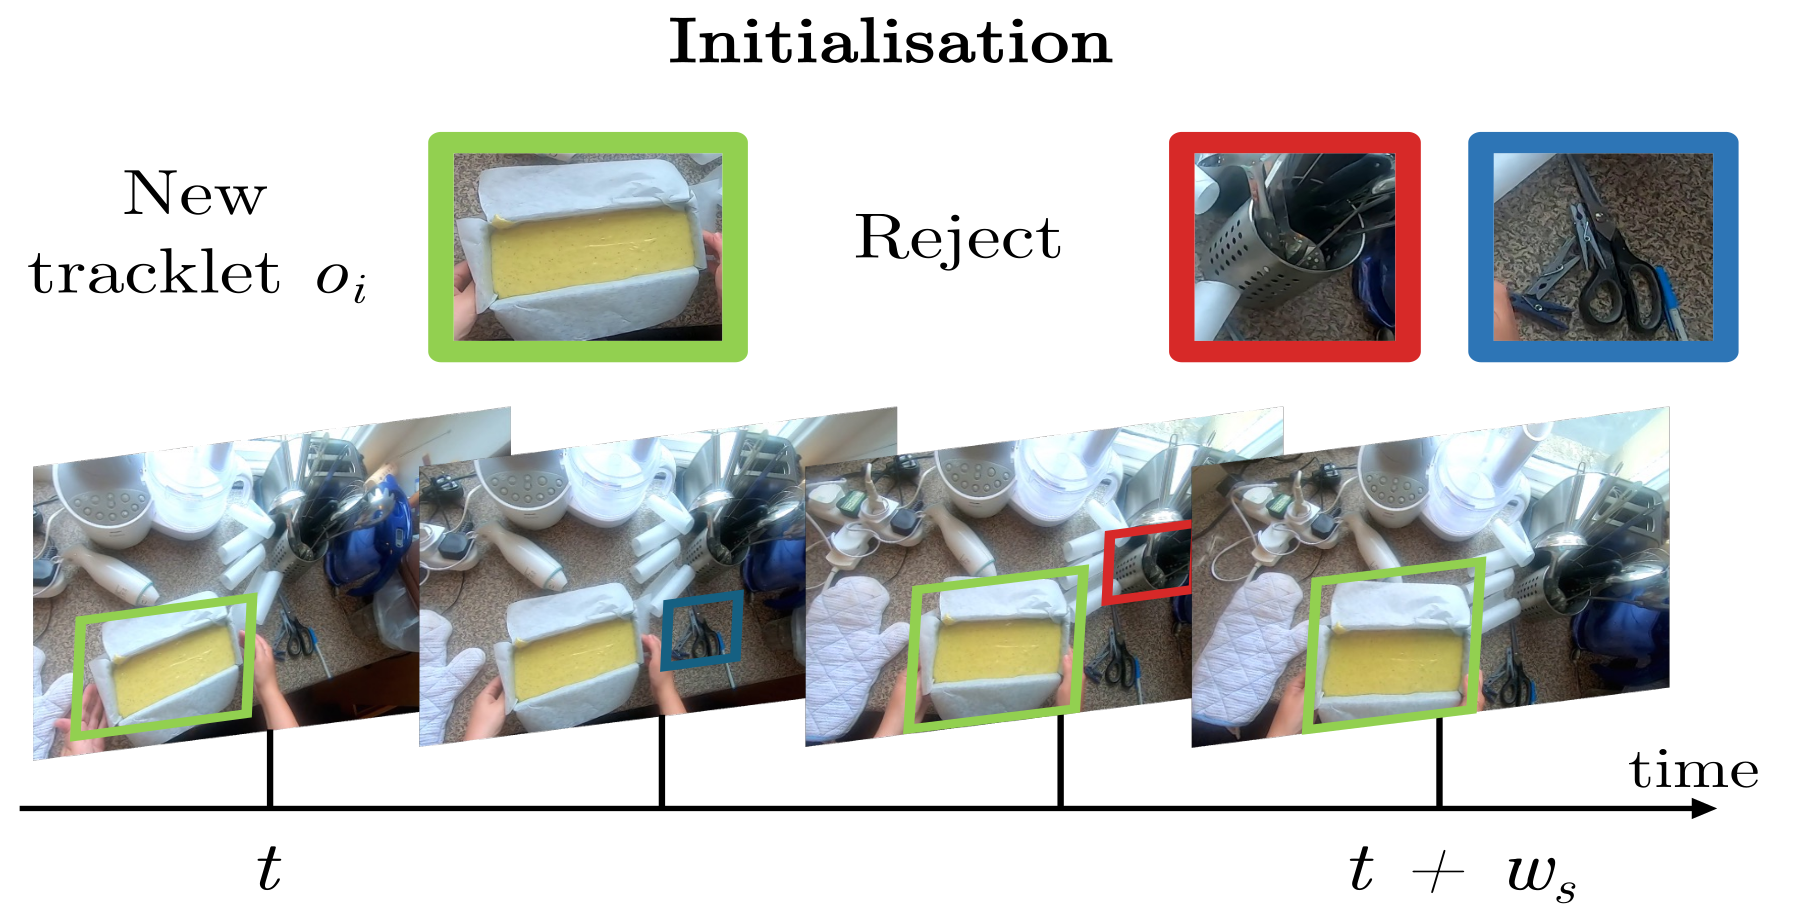
\includegraphics[width=0.6\textwidth]{Images/init.png}
    \caption{Fase di inizializzazione}
    \label{fig:init}
\end{figure}

Questo filtraggio spazio-temporale permette di ridurre il rumore derivante dall’applicazione indipendente del rilevatore su ciascun frame. Considerando la durata naturale delle interazioni mano-oggetto, è possibile identificare in modo affidabile i nuovi tracklets attivi, garantendo coerenza spaziale e temporale nelle rilevazioni.  

Il tracklet $o_i$ viene ora considerato \emph{attivo} e aggiunto alla memoria $\mathcal{O}$.  

Per ciascun frame successivo, calcoliamo l’\emph{Intersection over Union (IoU)}\footnote{\textbf{Intersection over Union (IoU)}: misura di sovrapposizione tra due bounding box, calcolata come il rapporto tra l'area di intersezione e l'area di unione dei due rettangoli.} tra i bounding box degli oggetti che interagiscono con la stessa mano. I bounding box che superano una soglia $\theta$ vengono assegnati al tracklet $o_i$. Se non è possibile assegnare nuovi bounding box al tracklet, questo viene considerato \emph{terminato}.

\subsection*{Updating}

Questa fase mira a catturare l’intera durata dell’interazione e contemporaneamente a seguire tutte le occorrenze spaziali dell’oggetto.

Sebbene i rilevatori di HOI a livello di singolo frame siano sufficienti per identificare nuove interazioni, essi non sono in grado di estendere in modo affidabile i tracklets quando mani o oggetti escono dal campo visivo egocentrico. Per questo motivo, viene utilizzato un off-the-shelf \emph{single-object tracker (SOT)}\footnote{\textbf{Single-Object Tracker (SOT)}: permette di seguire un singolo oggetto nel tempo, stimandone la posizione frame per frame anche in assenza di rilevazioni dirette.} \cite{tang2023egotrackslongtermegocentricvisual}.  

\begin{figure}[ht]
    \centering
    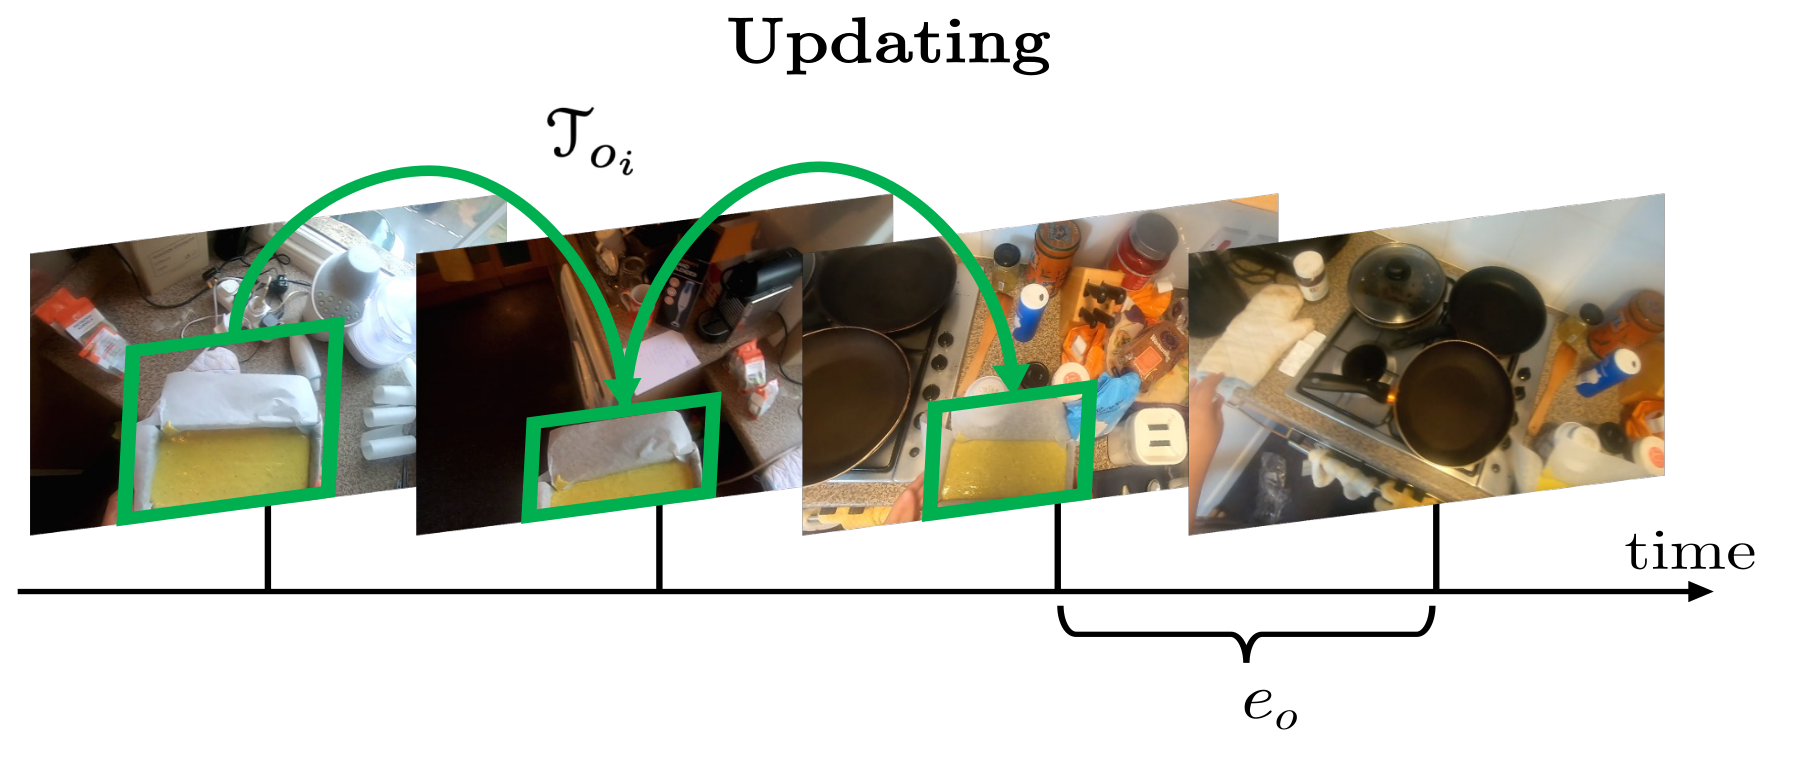
\includegraphics[width=0.6\textwidth]{Images/update.png}
    \caption{Fase di updating}
    \label{fig:update}
\end{figure}

Per ogni tracklet attivo $o_i$ viene inizializzato un SOT. Consideriamo il tracklet $o_i$ terminato se non sono presenti rilevazioni associate $\mathcal{B}^o$ per $e_o$ frame consecutivi, mentre la mano $h$ rimane visibile, in quanto quando la mano esce dal campo visivo è probabile che stia ancora tenendo l’oggetto.

L’output del SOT produce un track $\tau_{o_i}$ spazio-temporale che segue la posizione dell’oggetto, ma non contiene informazioni sull’interazione stessa. A questo punto, $o_i$ combina le informazioni relative alla durata temporale (start e end time) e ai bounding box spaziali dell’oggetto attivo, sfruttando sia la rilevazione HOI a livello di frame sia il tracciamento SOT.

\subsection*{Assignment and storing}

Come definito in precedenza, ogni HOI tracklet $o_i$ deve essere associato a una specifica istanza di oggetto. Per farlo, confrontiamo $o_i$ con le istanze già presenti nella memoria.  

In particolare, data l'insieme di HOI tracklets già memorizzati al tempo $t$, denotato $\mathcal{O}_t$, e l'insieme dei tracciamenti SOT osservati nello stesso istante, $\tau_t$, verifichiamo se $o_i$ possa essere associato a un'istanza esistente o se sia necessario crearne una nuova. Per effettuare il confronto, calcoliamo prima le feature visive di $o_i$:

\[
f(o_i) = \frac{1}{|\mathcal{V}_{o_i}|} \sum_{k \in \mathcal{V}_{o_i}} \gamma(k, b_k^o)
\]

dove:
\begin{itemize}
    \item $\mathcal{V}_{o_i}$ è l'insieme dei frame associati a $o_i$,
    \item $b_k^o$ è il bounding box relativo al frame $k$,
    \item $\gamma$ visual-feature-extractor (nel nostro caso DINOv2 \cite{oquab2024dinov2learningrobustvisual}).
\end{itemize}

Per effettuare il \emph{matching}, utilizziamo un approccio di clustering online basato su $f(o_i)$. La similarità tra $o_i$ e una specifica istanza di oggetto $id_j$ viene calcolata come:

\[
s(o_i, id_j) = \frac{1}{|\mathcal{O}_t \in id_j|} \sum_{\mathcal{O}_t \in id_j} \langle f_{\mathcal{O}_t}, f_{o_i} \rangle
\]

dove $\langle \cdot, \cdot \rangle$ indica la \emph{cosine similarity} e $\mathcal{O}_t \in id_j$ è l'insieme dei tracklets associati all'istanza $id_j$.  

Assegniamo $o_i$ all'istanza $id_j^*$ che massimizza la similarità e che supera una soglia $\theta$ (diversa dalla soglia utilizzata per l'IoU). Se un tracker in $\tau_t$ si sovrappone significativamente con $o_i$ e la sua confidenza è maggiore della similarità massima, allora $o_i$ viene assegnato all'istanza del tracker. Altrimenti, viene assegnato a $id_j^*$. Qualora la similarità massima risultasse inferiore alla soglia, viene creata una nuova istanza per $o_i$.  

Al termine di questa fase, le feature $f(o_i)$ e l'istanza assegnata vengono associate al tracklet $o_i$ e memorizzate nella memoria $\mathcal{E}$

\subsection{Location segments}
Definiamo l'insieme dei \emph{Location segments} $\mathcal{L}$ come gli intervalli temporali durante i quali il soggetto svolge interazioni in \emph{zone di attività principali}

Poiché un soggetto può interagire con più oggetti simultaneamente ma può trovarsi in un solo punto alla volta, ogni segmento $l_i \in \mathcal{L}$ viene modellato come un intervallo temporale che corrisponde all'inizio e alla fine di un'interazione in quella specifica zona.  

Analogamente agli \emph{HOI tracklets}, l'insieme $\mathcal{L}$ viene costruito online.

Si seguendo due fasi principali: Temporal segmentation e Assignment and storing

\subsection*{Temporal segmentation}
Dati i frame $\mathcal{V}_t$ e le rilevazioni delle mani $B_t^h$, verifichiamo se la mano sta interagendo con un oggetto mentre si trova in una location. Per farlo, calcoliamo l'\emph{optical flow}\footnote{\textbf{Optical flow}: rappresenta il campo di movimento apparente dei pixel tra due frame consecutivi di un video, indicando la direzione e la velocità dello spostamento}tra $\mathcal{V}_{t-1}$ e $\mathcal{V}_t$ e controlliamo la presenza di mani assicurandoci che $|B_t^h|>0$.

Possiamo quindi determinare se il soggetto sta svolgendo un compito considerando le seguenti condizioni:
\begin{enumerate}
    \item l'\emph{optical flow} ha norma\footnote{\textbf{Norma}: grandezza che rappresenta l'intensità complessiva di un vettore, nel nostro caso l'optical flow} bassa;
    \item è rilevata almeno una mano.
\end{enumerate}
Questi criteri permettono di stabilire se il soggetto ha fatto una pausa (basso \emph{optical flow}) ed è attivamente coinvolto nella scena (mano rilevata).

Analogamente agli HOI, applichiamo un filtraggio temporale, per cui un \emph{Location segment} $l_j$ è considerato attivo solo se entrambe le condizioni sono verificate per un numero consecutivo di frame $s_l$. Il segmento $l_j$ viene terminato quando osserviamo un numero consecutivo di frame $e_l$ in cui la norma dell'\emph{optical flow} supera la soglia o non sono presenti mani rilevate.

\subsection*{Assignment and storing}
Come per gli HOI, dobbiamo assegnare un'istanza alle location $l_j$ definite temporaneamente. Agiamo analogamente, utilizzando però un \emph{visual-feature-extractor} differente, $\sigma$ (SWAG)\cite{singh2022revisitingweaklysupervisedpretraining}.

Una volta ottenute le visual-feature $g_{l_j}$, calcoliamo la similarità tra tutte le istanze di location già presenti e assegniamo a $l_j$ l'id che massimizza questa similarità, a condizione che superi una soglia prestabilita $\tau$. Se la soglia non viene superata, viene creata una nuova istanza.

\[
s(l_j, id_j) = \frac{1}{|\mathcal{L}_t \in id_j|} \sum_{\mathcal{L}_t \in id_j} \langle g_{\mathcal{L}_t}, g_{l_j} \rangle
\]

Al termine di queste fasi, assegniamo $g(l_j)$ e l'istanza correlata nella nostra memoria $\mathcal{E}$.

\section{Pseudocode}

Di seguito vengono riportati i pseudocodici relativi alla costruzione della pipeline per la generazione degli elementi della memoria discussi nei paragrafi precedenti.

\subsection{Object interactions}
\begin{algorithm}[H]
\caption{Object interactions pipeline}
\begin{algorithmic}[1]
\State \textbf{Input:}
\State \quad Frames $\{V_t\}$
\State \quad HOI detector $\mathcal{D}$
\State \quad SOT tracker $\mathcal{J}$
\State \quad Similarity threshold $\theta$
\State \textbf{Output:}
\State \quad Set of hand-object interaction tracklets $\mathcal{O}$
\For{each frame $V_t$ do}
\State \quad $\mathcal{B}_t^o, \mathcal{B}_t^h \gets \mathcal{D}(V_t)$ (Detect hands and objects)
\For{each detection $(b^o, b^h) \in (\mathcal{B}_t^o, \mathcal{B}_t^h)$ do}
\If{new hand-object interaction (i.e. so detections in the last $w_s$ frames) then}
\State \quad \quad Create new tracklet $o_i$
\State \quad \quad Start SOT $\mathcal{J}_{o_i}$ for $o_i$
\EndIf
\EndFor
\For{each tracklet $o_i$ do}
\State \quad Update the detections with $\mathcal{J}_{o_i}$
\If{$\exists \tilde{b}^h \in \mathcal{B}_t^h$ matching with $o_i$ in the last $e_o$ frames and $|\tilde{b}^h|>0$ then}
\State \quad \quad Mark $o_i$ as complete
\EndIf
\EndFor
\EndFor
\For{each completed tracklet $o_i$ do}
\State \quad Compute visual features $f(o_i)$ (Eqn. 1)
\State \quad Compute similarity $s(o_i, id_j)$ with existing instances in $\mathcal{O}$ (Eqn. 2)
\If{maximum similarity $>\theta$ then}
\State \quad \quad Assign $o_i$ to best matching instance $id_j$
\Else
\State \quad \quad Create new instance for $o_i$
\EndIf
\State \quad Store $o_i$ in $\mathcal{O}$
\EndFor
\State \textbf{return} $\mathcal{O}$
\end{algorithmic}
\end{algorithm}
\subsection{Location Segment}
\begin{algorithm}[H]
\caption{Location Segment pipeline}
\begin{algorithmic}[1]
\State \textbf{Input:}
\State \quad Frames $\{V_t\}$
\State \quad HOI detector $\mathcal{D}$
\State \quad Similarity threshold $\tau$
\State \textbf{Output:}
\State \quad Set of location segments $\mathcal{L}$
\For{each frame $V_t$ do}
\State \quad $\mathcal{B}_t^o, \mathcal{B}_t^h \gets \mathcal{D}(V_t)$ (Detect hands and objects)
\State \quad Compute optical flow OpticalFlow($V_{t-1}, V_t$)
\If{location segment $l_j$ is active then}
\If{high $|\text{OpticalFlow}(V_{t-1}, V_t)|$ or $|\mathcal{B}_t^h| = 0$ for $e_l$ consecutive frames then}
\State \quad \quad Mark $l_j$ as complete
\Else
\State \quad \quad Continue $l_j$
\EndIf
\Else
\If{low $|\text{OpticalFlow}(V_{t-1}, V_t)|$ and $|\mathcal{B}_t^h| > 0$ for $s_l$ consecutive frames then}
\State \quad \quad Subject is interacting, start active location segment $l_j$
\EndIf
\EndIf
\EndFor
\For{each completed segment $l_j$ do}
\State \quad Compute visual features $g(l_j)$
\State \quad Compute similarity $s(l_j, id_i)$ with existing instances in $\mathcal{L}$
\If{maximum similarity $>\tau$ then}
\State \quad \quad Assign $l_j$ to best matching instance $id_i$
\Else
\State \quad \quad Create new instance for $l_j$
\EndIf
\State \quad Store $l_j$ in $\mathcal{L}$
\EndFor
\State \textbf{return} $\mathcal{L}$
\end{algorithmic}
\end{algorithm}


\section{AMB - Active Memories Benchmark}
Per studiare l'interazione tra oggetti attivi, location e la loro correlazione. è stato introdotto un benchmark ad-hoc, l'\emph{Active Memories Benchmark} (AMB).

Il benchmark comprende 20.500 query che coprono diversi livelli di ragionamento. Le query sono formulate come domande a scelta multipla.

Ad esempio, alcune domande riguardano l'utilizzo di oggetti: ``Quale oggetto ho usato con [VQ]?'' dove [VQ] rappresenta un ritaglio visivo dell'oggetto; altre domande chiedono ``In quali location ho usato [VQ]?''

\begin{figure}[ht]
    \centering
    \includegraphics[width=1\textwidth]{Images/benchmark.png}
    \caption{Esempi di query del benchmark AMB.}
    \label{fig:benchmark_queries}
\end{figure}

Come si nota, nelle domande non compaiono i nomi degli oggetti. Ogni visual query di un oggetto (VQ), risposta visiva dell'oggetto (VA), query sulla location (LQ) o risposta sulla location (LA) è parametrizzata tramite patch visive.

\subsection{Tipologie di query}

Le query sono strutturate in tre macro aree:
\begin{itemize}
    \item \textbf{\textcolor{sqcolor}{Sequencing (SQ) [Q1-4]}}: valutano la capacità di discriminare l'ordine temporale degli eventi. Ad esempio, il modello deve ordinare le interazioni nel tempo e identificare quale oggetto è stato utilizzato prima o dopo un altro.
    
    \item \textbf{\textcolor{cocolor}{Concurrency (CO) [Q5-6]}}: valutano la capacità di catturare interazioni multiple simultanee. Ad esempio, verificare se diversi oggetti sono stati utilizzati insieme (oggetto-oggetto) o se un oggetto è stato usato in una specifica location (oggetto-location).
    
    \item \textbf{\textcolor{tgcolor}{Temporal Grounding (TG) [Q7-8]}}: valutano la capacità di recuperare tutti gli intervalli temporali in cui un oggetto o una location è stato coinvolto in interazioni.
\end{itemize}

\begin{table}[ht]
    \centering
    \scriptsize % font più piccolo
    \setlength{\tabcolsep}{4pt} % riduce lo spazio tra colonne
    \begin{tabular}{|p{1.8cm}|p{1cm}|p{7.5cm}|p{1cm}|p{1.5cm}|p{1cm}|}
    \hline
    \textbf{Reasoning} & \textbf{Query} & \textbf{Template} & \textbf{Dim.} & \textbf{Answer} & \textbf{Qs} \\
    \hline
    \multirow{4}{*}{\textcolor[HTML]{789ECC}{SQ}} & \textcolor[HTML]{789ECC}{Q1} & What is the correct sequence of objects I have interacted with? & O & Obj. seqs & 464 \\
    \cline{2-6}
    & \textcolor[HTML]{789ECC}{Q2} & What did I use with the left/right hand after [VQ]? & O & Obj. & 3466 \\
    \cline{2-6}
    & \textcolor[HTML]{789ECC}{Q3} & What did I use with the left/right hand before [VQ]? & O & Obj. & 3466 \\
    \cline{2-6}
    & \textcolor[HTML]{789ECC}{Q4} & Where did I take/leave [VQ]? & O, L & Loc. & 1266 \\
    \hline
    \multirow{2}{*}{\textcolor[HTML]{C23A21}{CO}} & \textcolor[HTML]{C23A21}{Q5} & What did I use with [VQ]? & O & Obj. sets & 2105 \\
    \cline{2-6}
    & \textcolor[HTML]{C23A21}{Q6} & Where did I use [VQ]? & O, L & Loc. sets & 2320 \\
    \hline
    \multirow{2}{*}{\textcolor[HTML]{02BF3D}{TG}} & \textcolor[HTML]{02BF3D}{Q7} & When did I use [VQ]? & O & Intervals & 2614 \\
    \cline{2-6}
    & \textcolor[HTML]{02BF3D}{Q8} & When did I visit [LQ]? & O, L & Intervals & 809 \\
    \hline
    \end{tabular}
    \caption{Tipologia di domande AMB con colonne colorate per Reasoning e Query.}
    \label{tab:amb_queries_colored}
\end{table}    

\subsection{Risposte alle Query}
\textcolor{red}{approfondire come si elabora la risposta alle query}

\section{Risultati}

AMEGO è stato valutato confrontandolo con diverse baseline comuni per il task di video-QA:
\begin{itemize}
    \item \textbf{Semantic-free QA (SF-QA)} utilizza modelli vision-language, come CLIP \cite{radford2021learningtransferablevisualmodels}, per mappare query, video e risposte nello stesso spazio di embedding. Le feature visive vengono estratte dai frame del video, dai patch delle query e dalle risposte, mentre le feature testuali provengono dalla domanda. L'embedding della query è ottenuto come media delle feature, e la risposta con la similarità più alta viene selezionata.
    
    \item \textbf{SF-QA (obj)} è una variante di SF-QA che include anche le feature visive degli oggetti attivi rilevati da \cite{shan2020understandinghumanhandscontact}.
    
    \item \textbf{Semantic QA (S-QA)} sfrutta "captioner" pre-addestrati per generare un sommario semantico del video. Si usano LaViLa \cite{zhao2022learningvideorepresentationslarge} per il video egocentrico e BLIP-2 \cite{li2023blip2bootstrappinglanguageimagepretraining} per i patch della query. Le caption vengono poi passate a LLaMA-2-7B \cite{touvron2023llama2openfoundation} per rispondere alle domande. Se il testo supera i 4096 token, viene sottocampionato.
    
    \item \textbf{Multi-round semantic QA (LLoVi)} \cite{zhang2024simplellmframeworklongrange} funziona in due round: prima sintetizza le caption del video alla luce della domanda, poi risponde alla query usando il sommario generato.
\end{itemize}

I risultati sono riportati per AMEGO si dividono in: AMEGO-S e AMEGO-L, a seconda della dimensione del visual feature extractor (ViT-S/B vs ViT-L).

\begin{table}[ht]
    \centering
    \caption{Accuracy (\%) sulle diverse query di AMB. Migliori valori in grassetto.}
    \resizebox{\textwidth}{!}{%
    \begin{tabular}{|l|c|c|c|c|c|c|c|c|c|}
    \hline
    \multirow{2}{*}{\textbf{Method}} & \multicolumn{4}{c|}{\textbf{SQ}} & \multicolumn{2}{c|}{\textbf{CO}} & \multicolumn{2}{c|}{\textbf{TG}} & \multirow{2}{*}{\textbf{Total}} \\
    \cline{2-9}
    & Q1 & Q2 & Q3 & Q4 & Q5 & Q6 & Q7 & Q8 & \\
    \hline
    Random & 20.0 & 20.0 & 20.0 & 20.0 & 20.0 & 20.0 & 20.0 & 20.0 & 20.0 \\
    \hline
    SF-QA & 13.7 & 21.6 & 22.5 & 26.8 & 22.1 & 31.9 & 23.7 & 26.2 & 22.0 \\
    SF-QA (obj) & 13.1 & 23.4 & 22.6 & 23.2 & 21.7 & 26.1 & 23.8 & 25.2 & 21.2 \\
    \hline
    S-QA (LaViLa) & 20.9 & 20.6 & 21.2 & 24.6 & 24.9 & 27.1 & 21.4 & 22.6 & 22.4 \\
    S-QA (BLIP-2) & 23.9 & 22.0 & 22.5 & 23.3 & 27.5 & 27.0 & 20.2 & 24.1 & 23.6 \\
    S-QA (LaViLa+BLIP-2) & 22.8 & 22.2 & 21.4 & 22.6 & 25.1 & 26.1 & 21.4 & 24.5 & 22.9 \\
    \hline
    LLoVi (LaViLa) & 21.1 & 20.2 & 20.8 & 21.0 & 21.2 & 20.3 & 20.5 & 21.6 & 20.8 \\
    LLoVi (BLIP-2) & 22.3 & 21.4 & 21.8 & 22.2 & 25.6 & 26.7 & 18.1 & 22.2 & 22.4 \\
    LLoVi (LaViLa+BLIP-2) & 22.8 & 21.9 & 21.5 & 24.6 & 25.3 & 26.5 & 18.5 & 19.8 & 22.6 \\
    \hline
    AMEGO - S & 32.0 & 35.1 & 34.8 & 35.8 & 24.7 & 37.8 & 33.6 & 44.3 & 33.8 \\
    AMEGO - L & \textbf{33.7} & \textbf{36.3} & \textbf{37.2} & \textbf{38.3} & \textbf{27.6} & \textbf{44.3} & \textbf{34.7} & \textbf{48.9} & \textbf{36.3} \\
    \hline
    \end{tabular}%
    }
\end{table}

Tutte le baseline ottengono risultati migliori sulle query relative alla \emph{concurrency}, probabilmente perché sfruttano pattern ricorrenti presenti nei dati di addestramento, ad esempio una padella spesso utilizzata sul piano cottura \cite{goletto2024amego}. Tuttavia, le performance complessive rimangono vicine alla soglia della scelta casuale.

AMEGO invece ottiene buoni risultati su tutte le tipologie di query, superando le baseline con un margine consistente (+12.7\%). La domanda in cui AMEGO mostra maggior difficoltà è Q5, a causa dei limiti attuali dei detector di interazione mano-oggetto nel predire oggetti multipli che interagiscono contemporaneamente con la stessa mano del soggetto.